\chapter{Functioneel Ontwerp}\label{ch:functioneel-ontwerp} % Chapter title

\label{funtioneelOntwerp} % For referencing the chapter elsewhere, use \autoref{ch:InOnderzoek}

Uit het onderzoek naar de tooling om de analyses te doen is naar voren gekomen dat de analyses tijd op de build server in beslag nemen die er eigenlijk niet is. Hiervoor is gekozen om van de build een snapshot te maken met daarin een lijst van de dependencies binnen het project met daarbij meta data als projectnaam, type, timestamp, GitHash. Deze snapshots kunnen in een later stadium worden geannalyseerd op een moment dat de server hier de tijd voor heeft.

Om het bovenstaande proces te ondersteunen moeten er dus een aantal modules worden ontworpen die ieder een deel van dit proces uitvoerd.
\begin{itemize}
    \item \textbf{VersionExtractionTool} VET hé
    \begin{itemize}
        \item \textbf{VET-SBT} Een SBT plugin die een lijst van de dependencies maakt en deze in database plaatst
        \item \textbf{VET-NPM} Een NPM plugin die een lijst extraheert vanuit de package.json en deze in een database plaatst
        \item \textbf{VET-DOCK} scanner voor docker images. ( latere zorg)
    \end{itemize}
    \item \textbf{API} centrale module om gegevens op te slaan, bewerken en weer te geven
    \item \textbf{Analysers}
    \begin{itemize}
        \item SBT ANALYSER: Analyser die een dependency file(build.sbt) opbouwd die genalyseerd kan worden middels de gevonden tools
        \item NPM ANALYSER: een tool om van de snapshot een dependency declaratie(package.json) te bouwen en vervolgens een analyse uit te voeren die weer in de database te zetten.
    \end{itemize}

    \item \textbf{portal} GUI module in de portal voor weergave van status en de daadwerkelijke gegevens over kwetsbaarheden
    \item
\end{itemize}



\section{Architectuur ontwerp}\label{sec:architectuur-ontwerp}
Uit de requirements blijkt dat de module moet samenwerken met een aantal systemen binnen EagleScience. in figuur~\ref{fig:UML-ComponentDiagram} is te zien dat de SOUP-API een centraal onderdeel is van de module. Het is verantwoordelijk voor verschillende taken die nodig zijn voor de informatie behoefte die de module moet weergeven.

\begin{figure}[bth]
    \myfloatalign
    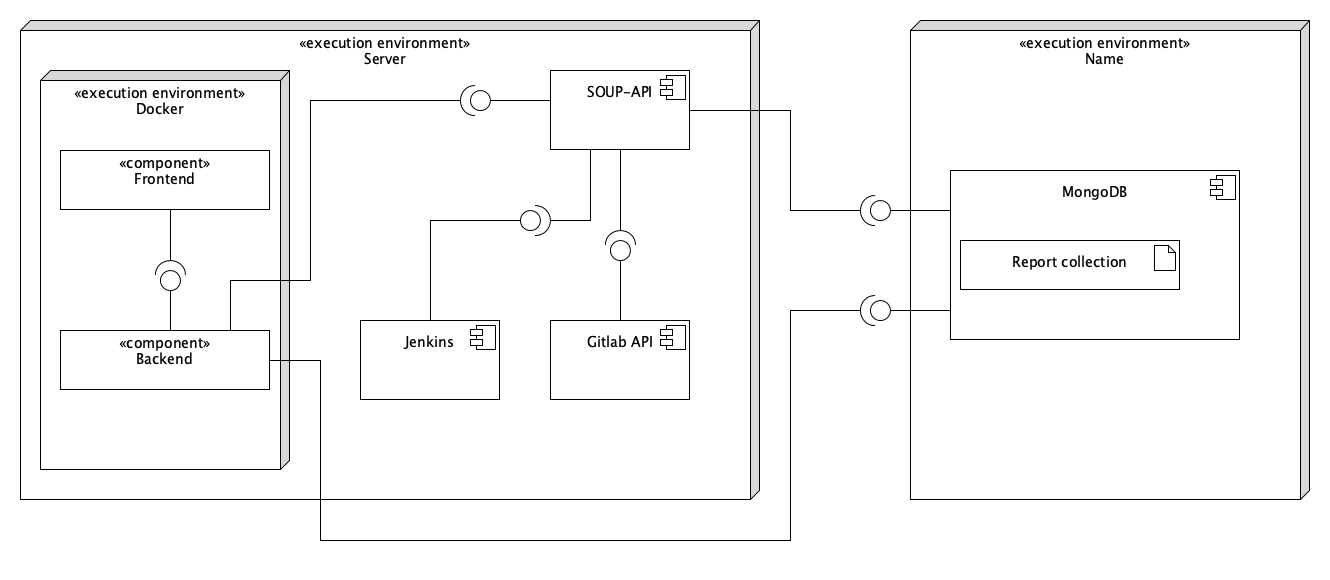
\includegraphics[width=15cm]{gfx/UMLcomponent diagram}
    \caption{Component diagram}
    \label{fig:UML-ComponentDiagram}
\end{figure}


\section{SOUP-API}\label{sec:soup-api}
Er \textbg{\textit{MOET}} nog een betere naam worden verzonnen.
DE SOUP-API is het centrale onderdeel van de module. Het heeft de functie rapporten te genereren. De generatie moet op twee momenten worden gedaan. Ten eerste als er nieuwe code in wordt gecheckt in Jenkins en ten tweede als een project al een tijd op productie draait moet er periodiek worden gecontroleerd of de gebruikte bibliotheken nog up-to-date en vooral veilig zijn.

\subsection{process: periodiek Checken van een repository op basis van nieuwe }\label{subsec:process:-periodiek-checken}
Er is een process nodig om periodiek een raport te genereren die inzicht geeft in de huidige staat van kwetbaarheden voor projecten.

\begin{enumerate}
    \item User doet POST request op "\textbackslash createreport?project="PROJECTNAAM"
    \item
\end{enumerate}


